\documentclass{article}
\usepackage{graphicx}
%\graphicspath{{photo}}
\begin{document}
\begin{figure}
\begin{center}
\textbf{Neha Dafedar}
\end{center}
\hrulefill\\
\begin{minipage}[t]{0.5\textwidth}
KLS GIT ,Udyambag\\
Belagavi--591108,\\
Karnataka\\
\end{minipage}
\begin{minipage}[t]{0.5\textwidth}
\raggedleft
contact:8147704246\\
email-id:nehadafedar786@gmail.com\\
\end{minipage}


\raggedleft
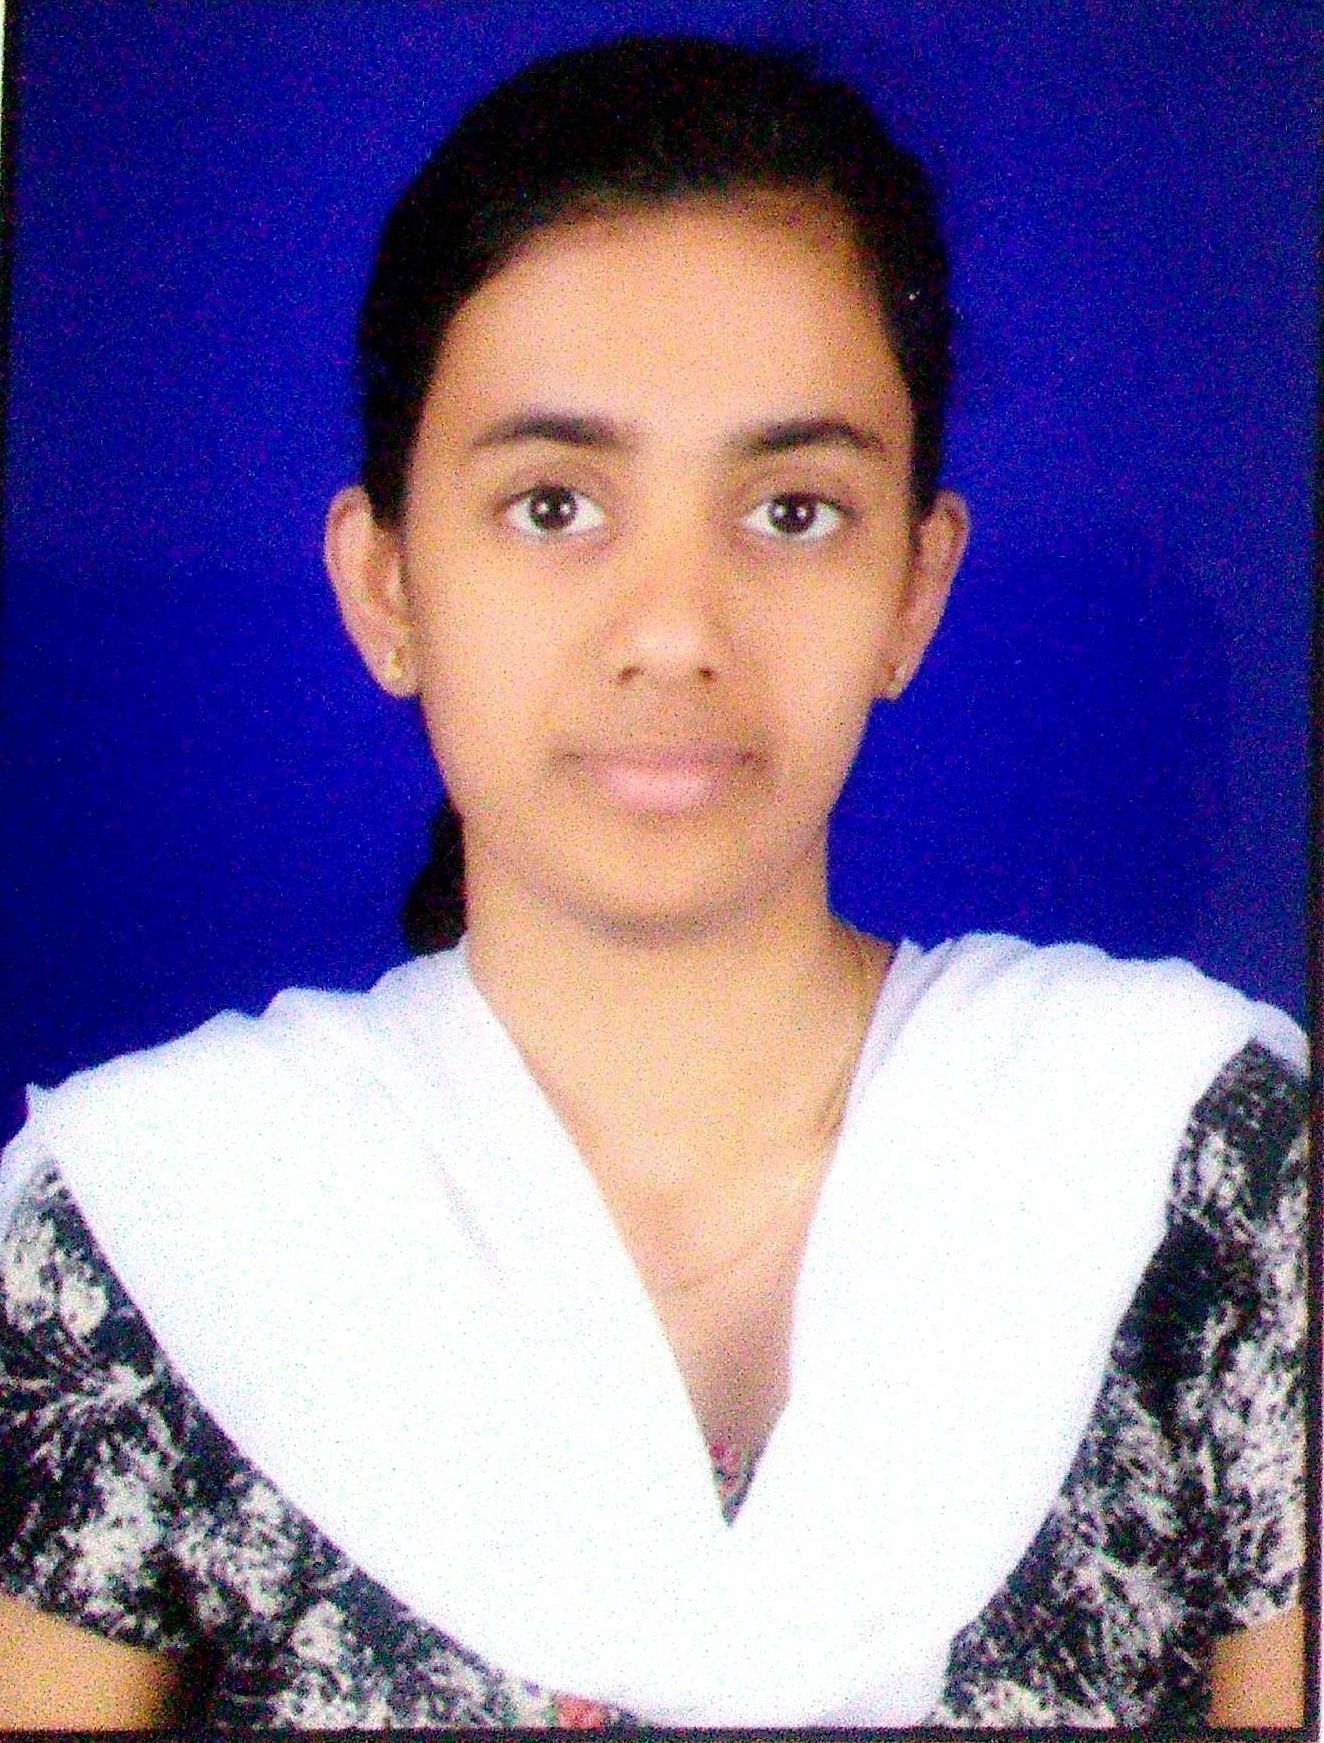
\includegraphics[width=20mm]{photo.jpg}
\end{figure}
\textbf{Objective}\\
 To percieve knowledge in the field of robotics and embedded systems.Seeking for an internship and job in the robotics and embedded field\\[0.5 cm]
\textbf{Education}\\[0.5cm]
\begin{tabular}{ l | c  | c | c | }
\textbf{Degree} & \textbf{School/College} & \textbf{Passing year} & \textbf{Passing percetage}\\ \hline
BE (ECE)& KLS Git Belagavi & 2018-19 & (current) cgpa 9.2\\ \hline
PUC 2 & KLE's BK college Chikodi & 2015 &  91.66\% \\ \hline
SSLC  & CTE society R D high school chikodi & 2013 & 91.5\% \\ \hline

\end{tabular}\\[0.5cm]
\textbf{Projects}\\[0.1cm]
\begin{enumerate}
\item\textbf{ Collector Bot:}Collector robot for picking and dropping fresh fruits using atmega2560.V-rep
software for simulation. Aruco markers for detecting aruco id and
differentiating fresh and damaged fruit.Python programming for simulation
and zigbee communication.
\item\textbf{Wheelchair}:It is a Arduino based prototype of wheelchair which can be easily controlled
using positioning the finger in the appropriate slot containing Proximity sensors.It also stops immediately
on the occurance of obstacle.
\item\textbf{Hamming codes:}Implementing error detecting and correcting hamming codes using MATLAB.
\item\textbf{Complex Multiplier:}Implementing complex number multiplier using HDL.\\[0.5cm]
\end{enumerate}
\textbf{Trainings}\\[0.1cm]
\begin{itemize}
\item\textbf{ VLSI }:Fath
IEEE online certification course started from  Apr 2017 till Jun 2017.
learnt verilog HDL programming
\item\textbf{BEC business english }:Conducted by Cambridge university from june 2016 to august 2016.
\item\textbf{Arduino Workshop}conducted by KLS Gogte Institute Of Technology Belagavi in 
May 2016 .
\item\textbf{Design Thinking Workshop}:conducted by KLS Gogte Institute Of Technology, Belagavi in Jan 2018.
\item\textbf{Web designing}:Basics of web desighning from coursera and codeacademy. \\
\end{itemize}
\end{document}